We have implemented the composable query processing architecture described in Chapter~\ref{ch:design_pattern} in the form
of a framework that facilitates the definition and deployment of QPU-based query processing systems.
We call the framework Proteus.
Proteus consists of:

\begin{itemize}
  \item A collection of implementations of QPU classes (Section~\ref{sec:proteus_qpu_architecture}).

  \item A service discovery mechanism that simplifies the configuration of a QPU architecture by allowing the QPU graph to self-organize
  with only local configuration input to each QPU instance (Section~\ref{sec:domain_dissemination}).

  \item An architecture description language that can be used to define the topology and configuration of QPU architectures
  (Section~\ref{sec:spec_language}).

  \item A mechanism for translating architecture descriptions to deployment plans (Section~\ref{sec:proteus_deployment}).
\end{itemize}

\noindent
In Section~\ref{sec:implementation}, we present the implementation details of Proteus.


\section{Query processing domain dissemination}
\label{sec:domain_dissemination}
The set of queries that a query processing unit can process constitutes its query processing \textit{domain}.
As presented in Section~\ref{sec:qpc_tree},
we encode the query processing domain using a tree data structure, called domain tree.

The domain of a query processing unit depends on its functionality (class), its configuration, and, in most cases,
on the domains of its downstream connections as well.
This is because QPU classes such as Join and Partition Manager process a given query by breaking it down to sub-queries,
sending these sub-queries to their downstream connections,
and then performing a computation over the returned results.
Essentially, a QPU of this type de-composes queries into simpler tasks, and delegates some of these tasks to their downstream connections.
Therefore, the set of queries that it can process depends on the types of tasks that its downstream connections can perform.

Because of that, a query processing unit requires the domain tree of each of its downstream connections for its operation.
More specifically, as presented in Section~\ref{sec:qpc_tree}, a QPU uses the downstream domain trees in order to:
(1) compute its own domain tree, and (2) generate downstream queries during query processing.
In this section, we describe the mechanism through which a query processing unit acquires the domain trees
of its downstream connections.

\subsection{Domain interface}
We extend the query processing unit specification with a mechanism that allows a QPU to request the domain trees of its connections.
For that, we define an additional interface, as follows:

\begin{displaymath}
  GetDomain() \rightarrow [(QPUClass, DomainTree)]
\end{displaymath}

An invocation of $GetDomain$ returns a stream that contains $DomainTree$ records, where $DomainTree$ is a serialization of a QPU's domain tree.
When a QPU receives an invocation of its domain interface, it establishes an output stream with the caller.
It then sends a $DomainTree$ record through the stream, representing its current domain tree.
Each time there is a change to the QPU's domain tree, it sends an additional $DomainTree$ record through the stream,
representing the updated domain tree.

Similarly to the query interface, $GetDomain$ requests follow the QPU graph topology:
An edge in the QPU graph from $QPU_A$ to $QPU_B$ indicates that $QPU_A$ can invoke the domain interface of $QPU_B$.

We define the domain interface response as a stream rather than an one-time response in order to enable propagation of
configuration, domain and topology changes through the QPU graph.
This is a first step towards enabling \textit{dynamic reconfiguration} of QPU architectures.
Examples of dynamic reconfiguration might include the creation new indexes or materialization of views at runtime.
We consider dynamic reconfiguration of QPU architecture out of the scope of this work.
It is, however, a direction for future work.

In order to support the domain interface, we extend the query processing unit specification with two additional methods:
a domain processor and a domain response processor.
These methods are analogous to the query interface methods.
The domain processor method is responsible for processing a GetDomain request,
and the domain response processor method is executed for each received domain response,
and is responsible for updating the QPU's local view accordingly.

\subsection{Query processing domain discovery mechanism}

The first task of the constructor of each query processing unit class is to initialize the QPU's domain tree.
For the Corpus Driver class this is performed using the input configuration (\S\ref{sec:qpc_tree}).
Every other QPU class, as discussed above, requires the domain trees of its downstream connections in order to compute its own domain tree.
Because of that, the constructor method of every QPU class except of the Corpus Driver starts by sending a $GetDomain$ request to each
of its downstream connections.
After receiving the corresponding responses, the constructor computes the QPU's domain tree, using the rules presented in Section~\ref{sec:qpc_tree}.

If a QPU receives a $GetDomain$ request while still this process is being performed, it creates the response stream,
but sends the response only after it has finished computing its domain tree.

We illustrate this process using the architecture shown in Figure~\ref{fig:domain_example_graph} as an example.
Figure~\ref{fig:domain_sequence_diag} depicts a sequence diagram that describes the message exchanges for domain discovery
in that QPU graph.
Upon initialization, the $Join$, $Selection_1$ and $Selection_2$ send a $GetDomain$ request to each of their downstream
connections,
$Corpus$ $Driver_1$ and $Corpus$ $Driver_2$ compute their query processing domains using their input configuration.
Once each $Corpus$ $Driver$ QPU computes its domain tree, it responds to the corresponding $GetDomain$ request.
When each $Selection$ QPU receives the $GetDomain$ response, it calculates its domain tree, and then it responds to the request from $Join$.
Finally, $Join$ receives the responses from $Selection_1$, $Selection_2$, and computes its domain tree.

The goal of the domain dissemination mechanism is to reduce the input configuration required by QPU instances,
in order to simplify the process of configuring and deploying a QPU architecture.
Thanks to this mechanism, the configuration of a query processing unit consists of ``local'' configuration
(configuration about that specific unit), as well as the endpoints of its downstream connections.
The QPU can then use the domain interface of its connections to obtain information about them.
For example, a Partition Manager connected to a number of Index QPU instances requires only the endpoints of its
connections as configuration.

\begin{figure}
    \centering
    \begin{minipage}{.3\textwidth}
        \centering
        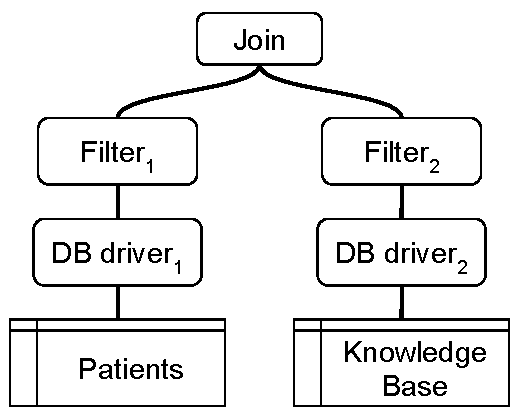
\includegraphics[scale=0.5]{./figures/design_pattern/qpu_graph_emergent_properties.pdf}
        \caption{An example QPU architecture.}
        \label{fig:domain_example_graph}
    \end{minipage}%
    \begin{minipage}{.7\textwidth}
        \centering
        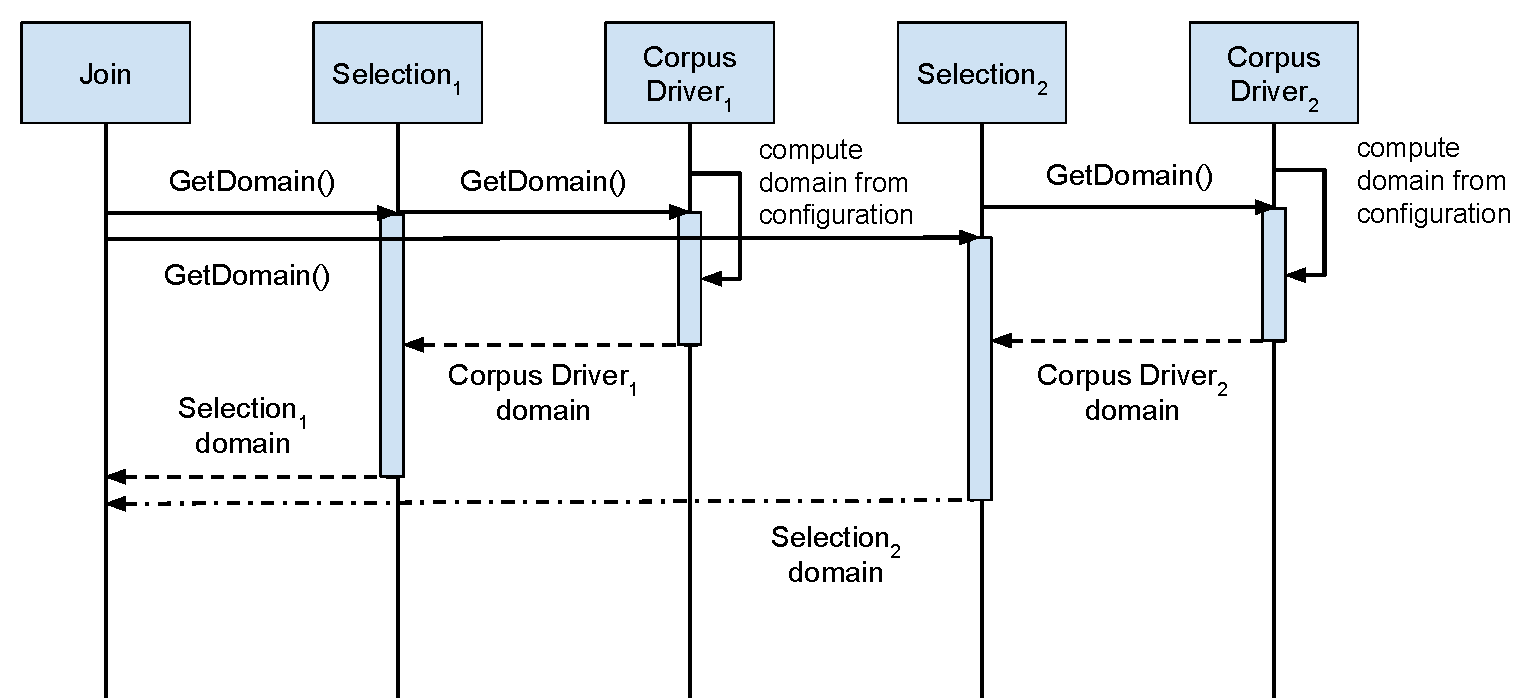
\includegraphics[scale=0.4]{./figures/proteus/domain_sequence_diag.pdf}
        \caption{Sequence diagram for the domain discovery of the architecture in Figure~\ref{fig:domain_sequence_diag}.}
        \label{fig:domain_sequence_diag}
    \end{minipage}
\end{figure}


\section{Query processing unit service}
\label{sec:proteus_qpu_architecture}
Proteus provides an implementation of the query processing architecture presented in Chapter~\ref{ch:design_pattern}.
We have implemented the query processing unit component as a service, i.e. a daemon process.
In this section we describe the system design and architecture of this service.

The design of the QPU service is guided by the principles of the query processing unit model.
Instead of implementing a separate QPU service for each QPU class,
we design the query processing unit service as a \textit{polymorphic} service:
Different instances of the same service implement different QPU classes, based on their configuration.
To achieve that, we separate the components that are common to every QPU class,
such as the configuration and query processing domain component,
and the components that are class-specific.
For the class-specific components, we provide implementations for different classes in the form a library.
We ensure that components are separated and communicate through well-defined APIs.

Our goal with this design is to make the query processing service \textit{extensible}.
Implementing an additional QPU class consists of extending the QPU class library with component implementations
for the additional class.

\subsection{QPU service architecture}

\begin{figure}
  \centering
    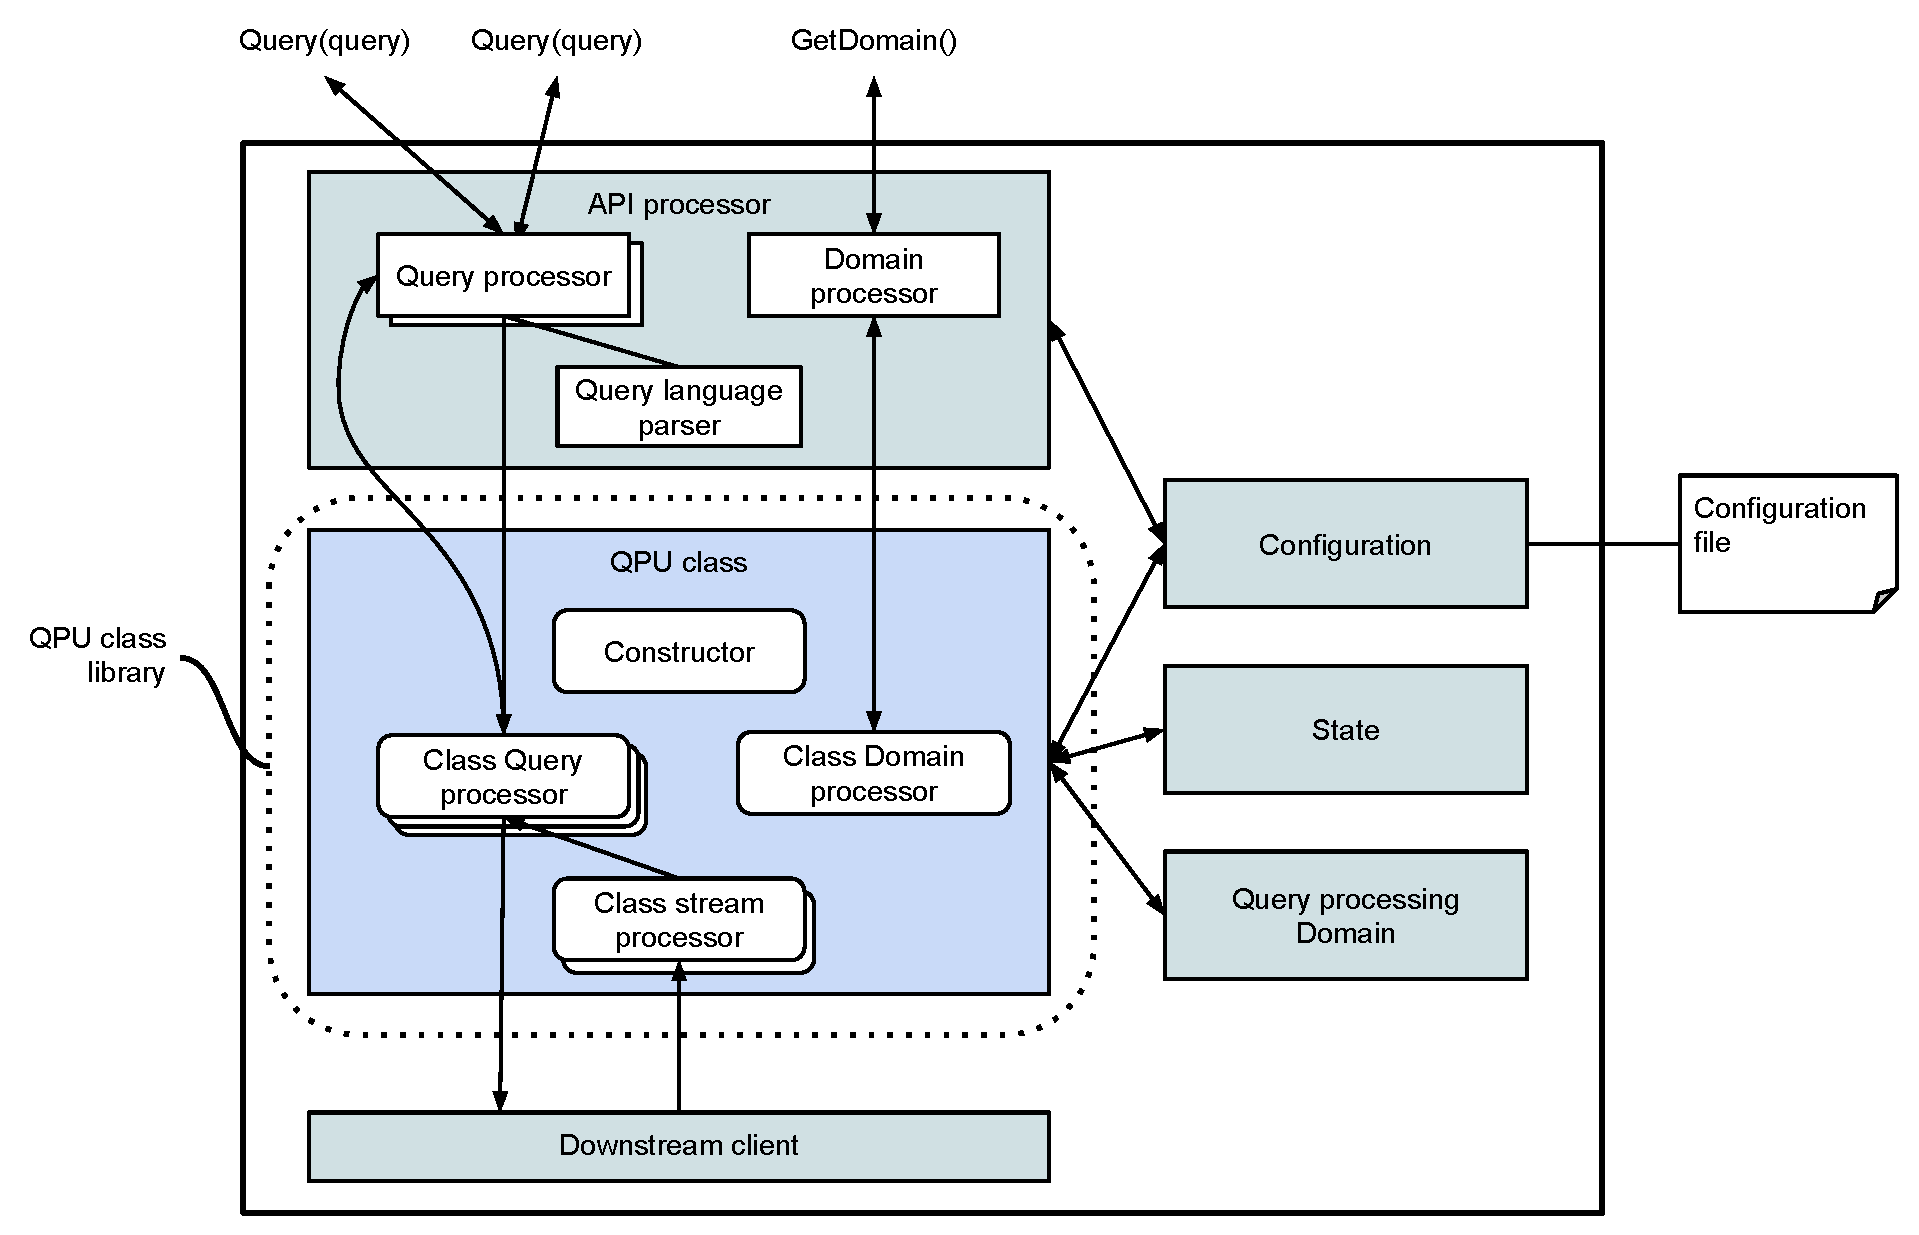
\includegraphics[width=0.7\textwidth]{./figures/proteus/QPU_architecture.pdf}
  \caption{An overview of the QPU service architecture.}
  \label{fig:qpu_arch}
\end{figure}

\medskip
\noindent
Figure \ref{fig:qpu_arch} depicts the components of the query processing unit service in Proteus.

A configuration file is passed to the QPU service during initialization.
The \textbf{Configuration} component is responsible for parsing the configuration file into a set of configuration parameters.
It exposes an API that other components can use to retrieve these configuration parameters.
Configuration parameters include the QPU class to be provided by the service,
the endpoints of downstream connections, and class-specific configuration parameters.
Some examples of class-specific configuration parameters are:

\begin{itemize}
  \item The Corpus Driver class configuration specifies endpoints of storage tier components that the Corpus Driver communicates with to provide its functionality,
  the table it is responsible for, and, optionally, the table's schema.

  \item The Index class configuration, as described in Section~\ref{sec:cs_index_partitioning},
  specifies an attribute name and an interval of values for that attribute.

  \item The Aggregator class configuration specifies an aggregation function, and the aggregation and grouping attributes.
\end{itemize}

\medskip
\noindent
The \textbf{Query Processing Domain} component is responsible for storing and providing access to QPU's domain tree as well
as the domain tree of downstream connections.
The QPU's domain tree is initialized by the QPU class Constructor method.
The domain trees of the QPU's downstream connections are initialized and subsequently updated by the QPU class Domain Response Processor.
The Query Processing Domain component provides two interfaces:
\begin{itemize}
  \item An interface for providing a serialization of the domain tree to the QPU class Domain processor, and
  \item An interface for computing downstream queries based on a given query parse tree.
\end{itemize}

\bigskip
\noindent
The \textbf{State} component is responsible for the QPU service's internal state.
It provides a key-value interface which other components use for storing and retrieving state entries.
The State component is used by derived state QPU classes, such as the Index and Materialized View classes,
for storing their derived state structures.

We have defined a key-value interface for the State component,
and have implemented multiple versions of the component using different backend stores:
an in-memory implementation using an ordered map data structure,
an implementation that uses MariaDB \cite{mariadb:docs} as backend store,
and one that use AntidoteDB \cite{antidotedb:docs}.
The State component to be used by a QPU service instance is controlled by a configuration parameter.

\bigskip
\noindent
The \textbf{API Processor} is responsible for receiving and processing incoming requests for the two open interfaces of
the query processing unit:
the Query and the Domain interface.
It provides a Query Processor method which is responsible for processing query requests,
and a Domain Processor method, responsible for domain requests.

When the Query Processor method is executed for query request received by the API processor,
it first parses the given query to a query parse tree \ref{sec:query_parse_tree} using the Query Language Parser.
If the query parse tree is successfully created, the Query Processor initiates a response stream,
and invokes the Class Query Processor of the QPU class specified in the configuration.
After executing the query, the Class Query Processor sends query result records back to the API Processor,
which emits them at the response stream.

Similarly, when the API Processor receives a GetDomain request,
it executes the Domain Processor, which passes the request to instance of the Class Domain Processor,
and emits each received response as a stream record.

The API Processor can process multiple requests concurrently.
For each received request, it creates an output stream,
and spawns the corresponding Processor method in a new thread.

\bigskip
\noindent
The \textbf{QPU Class} component is responsible for providing the methods defined by the query processing
unit specification (Sections~\ref{sec:QPU_model} and~\ref{sec:domain_dissemination}).
It is implemented as a library that provides QPU class method implementations.
Each class in the library provides five method definitions:
a Constructor method, a Class Query Processor method, a Domain Processor method, a Query Response Processor method,
and a Domain Response Processor method.
In our prototype, we have implemented the following QPU classes:
\begin{itemize}
  \item \textbf{Selection, Aggregation, Secondary Index, Partition Manager, Join, and Materialized view} as defined in previous chapters.

  As an optimization, we have integrated the functionality of the Selection class to other classes,
  such as the Corpus Driver, Secondary Index and Cache.
  This is because the Selections QPUs are often connected to these classes in QPU architectures.
  By integrating the selection functionality with these classes, we simplify QPU architectures
  and reduce the overhead of message serialization and de-serialization.

  Furthermore, in our current implementation, a Secondary Index QPU service is responsible for a single attribute in a single
  continuous value interval, specified by its configuration.
  A multi-attribute query is decomposed into a conjunction of multiple single attribute queries.

  \item \textbf{Cache}.
  We have implemented a Cache QPU class that stores query responses in an in-memory ordered map data structure.
  It uses a Least Recently Used eviction policy.
  Moreover, we defined the cache size in terms of \textit{query result records}.
  That is, a query result that contains $N$ data items occupies $N$ units of cache size.

  Moreover, we have implemented a time-based and an notification-based invalidation policy.
  In the time-based policy, cache entries are invalidated after an amount of time specified by the QPU's configuration.
  In the notification-based policy, the Cache QPU performs, for each query,
  a downstream persistent query to subscribe to notifications for updates that modify the query result;
  When a query result changes, the Cache QPU invalidates the corresponding cache entry.
  The invalidation policy is controlled by a configuration parameter.

  \item \textbf{Aggregator.}
  We have implemented a generic Aggregator Class that divides an input set of data items into groups based on a grouping attribute,
  and applies a function over an aggregation attribute to the data item of each group.
  The grouping and aggregation attributes as well as the aggregation function are configuration parameters.
  An aggregation operation fails if any data item in the input does not have a value for  the grouping or the aggregation attribute.
  Our current implementation provides the sum and count functions.

  \item \textbf{Corpus Driver.}
  We have implemented three versions of the Corpus Driver class, corresponding to different storage systems.:
  a relational database (MySQL \cite{mysql:docs}), a key-value store (AntidoteDB \cite{antidotedb:docs}),
  and an object storage system (Scality's CloudServer \cite{cloudserver:github}).
  We present more details on the implementation of each Corpus Driver in Section~\ref{sec:implementation}.

  \item \textbf{Network.}
  We have defined and implemented an additional class, called Network.
  A Network QPU has a single downstream connection.
  It forwards every received query request to that connection, and then forwards the input stream as its output stream.
  Moreover, it can be configured to delay, re-order or drop stream records, based on a specified distribution.
  The goal of this class is to simulate various network conditions for testing purposes.

  % \item \todo{TODO: Query Router}

\end{itemize}

The QPU class library is extensible;
Additional classes can be implemented by providing the corresponding method definitions.

\bigskip
\noindent
The \textbf{Downstream client} component is responsible for sending downstream requests to other QPU services.
It exposes an interface other components can use to submit query and domain requests.
The Downstream clients sends these requests to the corresponding connections,
and for each received response records it invokes the corresponding Class Response Processor method.

Moreover, the Downstream client component is responsible for delivering the records of a each stream exactly once and in-order
to the QPU Class.
To achieve this, the API processor assigns a sequence number to each emitted stream record.
The Downstream client uses these stream numbers to determine if records have been lost, already received or re-ordered.
Moreover, the Downstream client can request from downstream connections to re-transmit records that it has missed,
using control messages in the stream.
The API Processor in turn stores stream records after sending them in a buffer of configurable length.


\section{Architecture specification language}
\label{sec:spec_language}
In this section, we present a simple architecture description language for describing QPU-based query processing architectures.

The goal of a an architecture description is to describe a QPU graph,
including the class and configuration of the QPUs at its vertices and the connections among them,
as well as the placement of the graph vertices across system nodes.

An architecture description comprises a series of placement context assignments,
a series of QPU instance declarations, and a series of declarations of connections between QPU instances.

A placement context is denotes a node or collection of nodes.
It has the following syntax:

\begin{lstlisting}[
  language=qpulang,
  caption={Syntax used for placement context assignment.},
]
PlacementCtx([endpoint], PlacementCtxName)
\end{lstlisting}

\noindent
where $[endpoint]$ is a collection of system nodes, expressed as hostnames, or IP addresses,
and $PlacementCtxName$ is the name of the context assigned to these nodes.
For example, the description:

\begin{lstlisting}[
  language=qpulang,
  caption={Assigning placement contexts to four nodes.},
]
PlacementCtx([10.200.4.56], "node_1")
PlacementCtx([10.200.3.45], "node_2")
PlacementCtx([10.200.4.56, 10.200.3.45], "dc_eu")
\end{lstlisting}

\noindent
assigns the node with address 10.200.4.56 to the context ``node\_1'' ,
the the node with address 10.200.3.45  to context ``node\_2'',
and both nodes to the context ``dc\_eu''.

\medskip
\noindent
A QPU context declaration has the following syntax:

\begin{lstlisting}[
  language=qpulang,
  caption={Syntax used for specifying the configuration of a query processing unit.},
]
Configuration = {
  config_parameter_1: value_1,
  config_parameter_2: value_2,
  ...
}

qpu_object = <QPU_class>(Configuration)
\end{lstlisting}

\noindent
where $<QPU\_class>$ denotes one of the classes available in the QPU library.
The configuration specifies the configuration parameters passed to the QPU during initialization.

\medskip
\noindent
Specifying a connection between QPUs has the following syntax:

\begin{lstlisting}[
  language=qpulang,
  caption={Syntax used for specifying a connection between two query processing units.},
]
qpu_object_1.connectTo(qpu_object_2)
\end{lstlisting}

\noindent
This defines that $qpu\_object\_1$ has a downstream connection to $qpu\_object\_2$.

\medskip
\noindent
Finally, the following syntax can be used to describe the placement of QPUs across system nodes:

\begin{lstlisting}[
  language=qpulang,
  caption={Syntax used for specifying the placement of a query processing unit},
]
qpu_object.place([PlacementCtxName])
\end{lstlisting}

\noindent
The $place$ method assigns a set of \textit{placement constraint} to query processing unit.
The QPU can be placed on any node that satisfies the constraint.
For example, based on the description:

\begin{lstlisting}[
  language=qpulang,
  caption={Creating two query processing units, and specyfing their placement on system nodes.},
]
PlacementCtx([10.200.4.56], "node_1")
PlacementCtx([10.200.4.56, 10.200.3.45], "dc_eu")

q1 = Selection(config_selection)
q2 = Cache(config_cache)

q1.place("node_1")
q2.place("dc_eu")
\end{lstlisting}

\noindent
$q1$ is placed on the node with address 10.200.4.56,
while $q2$ can be placed on either of the two nodes.

\bigskip
\noindent

A limitation of this configuration language is that it does not explicitly express the placement of a QPU graph
relative to the corpus and the client,
but rather it expresses placement on system nodes.


\section{Query processing system deployment}
\label{sec:proteus_deployment}

We have designed a Deployment Generator component in Proteus for translating QPU architectures defined using the configuration
language presented in the previous section into deployment plans.

Each QPU service runs in a Docker \cite{docker} container.
The Deployment Generator translates an architecture description into (1) a Docker Swarm stack file
and (2) a configuration file for each QPU service.
The architecture is then deployed using Docker Swarm \cite{docker:swarm}

Docker Swarm uses Compose files \cite{docker:composefile} as deployment specification files.
A Compose file is a YAML \cite{yaml} file defines a set of services, a service being defined as a set of replicas of container that share the same image.
The Deployment Generator creates a Compose file that defines a service for each QPU instance defined in the architecture description.
A configuration file is passed to each service, using a shared volume.
Moreover, the Deployment Generator specifies a common network that all QPU services are connected to.

In order to generate the configuration file to be passed to each QPU service, the Deployment Generator translates the configuration parameters
of each QPU instance in the architecture specification to a TOML \cite{toml} file.
Moreover, it adds to the configuration parameters the QPU instance's downstream connections as defined in the architecture specification.

% \section{Fault tolerance}
% Describe the mechanisms provided by Proteus for tolerating faults during query
% processing.
% \begin{itemize}
%   \item Lost or re-ordered stream records.
%   \item Mid-query QPU crash.
%   \item Partitions.
% \end{itemize}

% \section{Implementation}
% Report on the implementation of different components of Proteus, including:
% \begin{itemize}
%   \item The framework used for communication between QPUs.
%   \item How streams are implemented.
%   \item ...
% \end{itemize}

\section{Implementation}
\label{sec:implementation}

The prototype implementation of Proteus consists of 13k lines of Go (v1.14).
The source code is available at \url{https://github.com/dvasilas/proteus}.

% It can operate on a single server or across a cluster of servers.

\bigskip
\noindent
\textbf{Interface.}
Applications interface with Proteus through a protocol buffer \cite{protobuf:docs} interface over gRPC (v1.31) \cite{grpc:docs}
gRPC is an remote procedural call (RPC) framework.
Using gPRC, a client process can directly call a method on a server process, on a different machine, as if it were a local object.
The workflow for using gPRC consists of defining a service, specifying its interface; methods that can be called remotely
and their parameters and return types.
gRPC uses protocol buffers as its interface description language.
We selected gRPC due to its support for streaming and bidirectional streaming RPCs,
and because it provides compiler plugins that can generate client- and server-side code based on a service definition.

Each query processing unit includes a gRPC server, as well as a gRPC client for communicating with other QPUs.
Client applications also need to implement gRPC clients.

\medskip
\noindent
We have additionally implemented two clients libraries, in Go and Java.
In the Go driver library, the operation of opening a connection to QPU actually opens and maintains a pool of connections
to that QPU.
Performing a query operations consists of requesting an idle connection, potentially opening a new connection if no idle
connections are available, or, if the maximum number of connections has been reached,  waiting until a connection becomes
available, performing the operation, and returning the connection to the pool.

\bigskip
\noindent
\textbf{Storage.}
Overall, query processing units maintain state either in memory, or persistently in AntidoteDB \cite{antidotedb:docs} or
MariaDB (v.10.3.27) \cite{mariadb:docs}.
However, currently not all QPU implementations support all three state backends.
For example, our Index QPU implementation supports both in memory and AntidoteDB,
while the Aggregator and Join QPU implementations support only MariaDB.
For QPU implementations that support more that one backends,
the backend by a QPU instance is specified by a configuration parameter.

\bigskip
\noindent
\textbf{Subscribe API (see models chapter for terminology).}
As described in Section~\ref{sec:storage_tier_api}, the data storage tier exposes a logical Subscribe API that can be
used for subscribing to notifications for data items updates.
We have implemented the Subscribe API in three data stores: MySQL/MariaDB, CloudServer, and AntidoteDB \cite{scality:cloudserver},
a REST server that compatible with the AWS S3 API, implemented by Scality.
As a results, Proteus currently can be used with a data storage tier provided by one of these data stores.

We note that MySQL/MariaDB and AntidoteDB can be used both as a QPU state backend and as a storage tier.
These two roles are independent:
A QPU graph may be used to provide materialized view on top of AntidoteDB,
and independent instances of AntidoteDB also be used for maintaining the state of QPUs in the graph;

\textbf{MySQL/MariaDB:}
We implement the Subscribe API using a user-defined function \cite{mariadb:udfs}, executed in response to a trigger \cite{mariadb:triggers}.
One the same machine as the MySQL instance, we run an executable, termed notification server,
that 1) implements a gRPC server, and 2) listens for socket connections.
For each MySQL table associated with Proteus, we install triggers that call a user-defined function for each modification to
the table.
For each record that is inserted or updated, the user-defined function encodes and sends a message to the notification
server through a socket connection.
Corpus Driver QPUs can subscribe to this update stream using the notification server's gRPC service.
The notification server is schema-agnostic; however, making a table available to Proteus requires installing the corresponding
triggers for that invoke the user-defined function.

\textbf{CloudServer}
CloudServer does not provide trigger or user-defined function mechanisms analogous to MySQL.
We have thus modified CloudServer adding a notification service provided by a gRPC server.
Our implementation consists of 300 lines of Node.js.
The source code is available at \url{https://github.com/dvasilas/cloudserver/tree/proto/proteus}.

\textbf{AntidoteDB}
Similarly to CloudServer, we have modified AntidoteDB adding a simple notification service that can be used by Corpus Driver QPUs.
The source code is available at \url{https://github.com/dvasilas/antidote/tree/proteus/log_propagation}.

\bigskip
\noindent
\textbf{Operator implementation.}
The implementation of the core QPU functionalities,
including relational operators (e.g. join, aggregation) and query processing data structures (e.g. secondary indexes,
materialized views) are fairly straightforward.
This is because update operations work in an incremental fashion,
processing records as they arrive.


In addition, we note that, despite the fact that the $Query()$ API allows for queries with fine-grained timestamps.
most QPU implementations currently support three more coarse query modes:
snapshot queries, persistent (or subscribe queries), and a combination of the two.
Snapshot queries are executed on the most recent snapshot, in a best-effort fashion,
and submitting a query request for an earlier snapshot returns an error.

A notable exception is the index QPU, in which we have implemented a versioned secondary index.
In the versioned secondary index,
each update creates a new version of the corresponding posting list.
The index maintains a configurable number of versions for each data item;
old versions are deleted to reduce memory/storage resource consumption.
The index QPU maintains its state either in memory or in AntidoteDB.

\bigskip
\noindent
\textbf{Multi-threading.}
Each QPU maintains two thread pools: one for executing query requests and one for processing input stream records.
Query requests and processing of input records are submitted as tasks to be executed by available threads.
Our benchmarking showed that using worker pools results in improved performance and stability,
especially in the implementations with MySQL backend,
We attribute this to having a bounded number of threads performing database transactions,
since our previous implementation was creating a new thread for each incoming request.

\bigskip
\noindent
\textbf{Packaging and deployment.}

As mentioned above, the query processing unit service is packaged as a Docker container.
This container is common for all QPU classes:
the QPU's class configuration is specified by a configuration file passed to the service at initialization,
Deploying a QPU service consists of deploying the QPU container
and providing the configuration file as a shared volume.

We use Docker Swarm for deploying a QPU graph:
A Docker compose file specifies the QPU services to be deployed, the configuration file to be passed to each service,
and the placement of each service.
